\subsection{Тесты RocksDB}

\subsubsection{Пермонас записи}

В данном подразделе проведём эксперименты по перфомансу записи в зависимости от способа организации SSTable и количества ядер предоставленных RocksDB. Сравнение проводится на виртуальной машине \ref{vm:first} во встроенном в RocksDB бенчмарке db\_bench \cite{dbbench}. При следующих настройках: 


\begin{lstlisting}[language=bash, numbers=none, upquote=true]
$ db_bench \
          >out
          --benchmarks=fillrandom \
          --db=/tmp/rocks-level\
          --key_size=16\
          --value_size=984\
          --num=+ 10^7 / threads_cnt \
          --compaction_style=merge_policy \
          --threads=threads_cnt;

\end{lstlisting}


Тут представлен больше псевдокод общий для всех запусков. Все конфигурации количества потоков и политики слияния (compaction\_style) запускаются на одном и том же число запросов случайной записи (с точностью на +-8).

В этом эксперименте мы будем тестировать перфоманс случайной записи в зависимости от количества ядер при разных политиках слияния.

compaction\_style, =0 - реализует рассмотренную выше Leveling Merge Policy, а =1 - некоторая universal compaction, которая согласно документации RocksDB\cite{rocksdbwiki} "иногда называется tiered" \ , т.е. эта политика некотрый аналог выше рассмотренной Tiering Merge Policy.


\begin{figure}[ht]
  \centering
  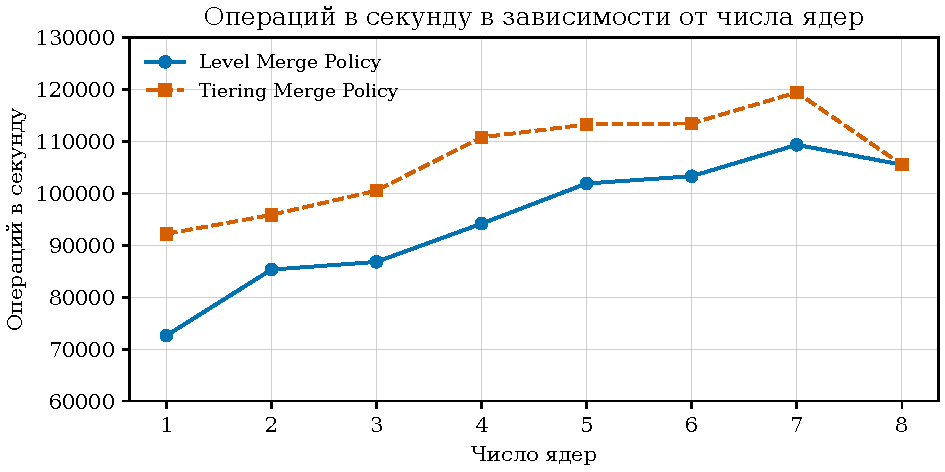
\includegraphics[width=\linewidth]{figures/04-01-ops-p-s-10-7.pdf}
  \caption{Число записей в секунду при $10^7$ операций случайной записи}\label{fig:intro-имя}
\end{figure}

Из графиков видно сразу несколько фактов:

Во-первых, не стоит отдавать СУБД все ядра системы, так как OS так же потребляет ресурсы компьютера, поэтому использование всех ядер ВМ \ref{vm:first} ведёт к снижению перфоманса.

Во-вторых, использование большего числа потоков записи всё ещё ведёт к увеличению числа операций, несмотря на необходимость синхронизации записи в LSMT (берём это как факт, т.к. так утверждают авторы статьи \cite{luo2020lsm}).

В-третьих, Tiering Merge Policy-подобная система хранения, действительно показывает лучший перфоманс записи, который уже на трёх ядрах работает сопоставимо быстро семи (и предполагаю даже 8ю, если бы данные не были испорчены ОС) ядрам в режиме Level Merge Policy. При 4 ядрах Tearing MP показывает уже превосходящий перфоманс записи, чем 7-8 ядер Level MP.
